\section{Trådløs kommunikation}
Den trådløse kommunikation er designet til direkte kommunikation mellem mikrokontrolleren og NXT'en til at styre exoskelettet. Herudover skal der etableres en trådløs kommunikation til en computer til debugging, test af mikrokontrolleren samt datavisualisering.   

\noindent
Til implementeringen af den trådløse kommunikation tages der ikke udgangspunkt i det oprindelige design. Dette er som følge af opsætningen af bluetooth kommunikationen i mikrokontrolleren, er fremkommet til at være mere kompliceret end først antaget. Dette omfatter, at der kræves en forståelse for diverse bluetooth programmeringsbiblioteker samt relaterede funktioner til at programmere buletooth kommunikation. For at implementere dette, vil den krævede tid således blive for lang og usikker i forhold til den endelige funktionalitet.
Dertil vælges det at implementere et mere simpelt og anvendeligt alternativ, bestående af to PSoC 4 M-Series Prototyping Kit board, der ses af \autoref{fig:PSoC_4200}

\begin{figure}[H]
	\centering
	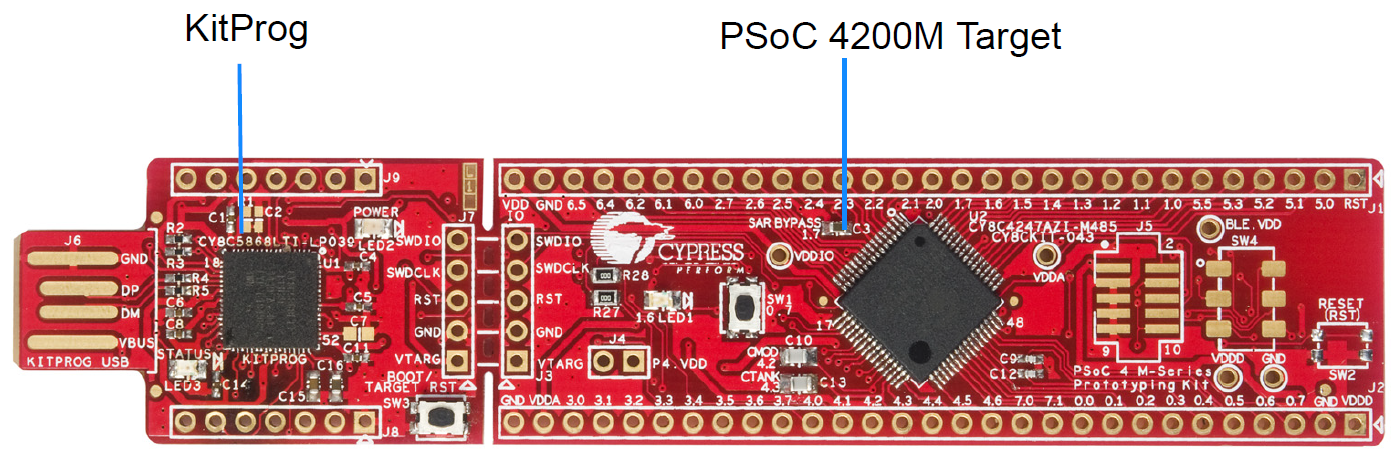
\includegraphics[width=0.8\textwidth]{figures/PSoC_4200_opdelt}
	\caption{CY8CKIT-043 PSoC 4 M-Series Prototyping Kit\citep{cypress42015}.}
	\label{fig:PSoC_4200}
\end{figure}

Dette board består af en KitProg og en PSoC 4200M enhed. KitProgen anvendes til at debugge og programmere koden. PSoc 4200M er processoren, hvorpå koden eksekveres. Yderligere er boardet udstyret med et EZ-BLE modul, der tillader trådløs kommunikation ved brug af bluetooth low energy. 
Den ene PSoC 4200M tilkobles mikrokontrollern via UART forbindelse og den anden tilsluttes computeren via USB og erstatter BLE donglen fra det oprindelige design. En illustration af, hvordan kommunikationen transmiteres i det implementerede system fremgår af \autoref{fig:Traadloes_Komm_Imp}.

\begin{figure}[H]
	\centering
	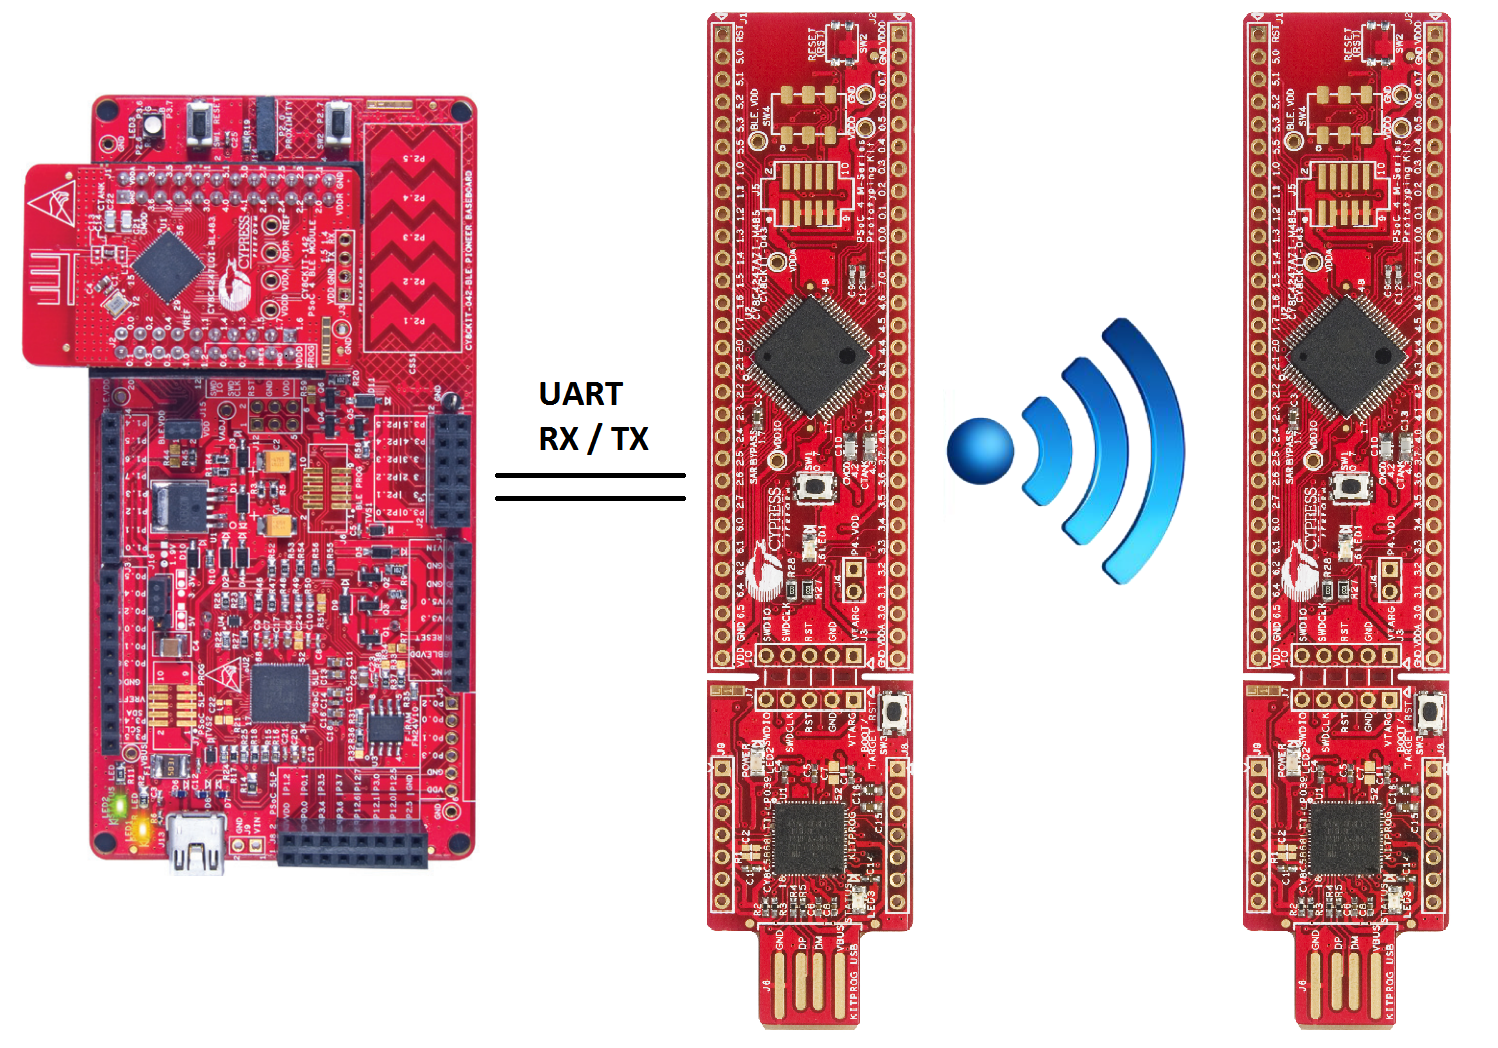
\includegraphics[width=0.8\textwidth]{figures/Traadloes_Komm_Imp}
	\caption{Illustration af kommunikation mellem mikrokontroller og computer. Der ses UART forbindelse til venstre, hvor der er anvendes RX (receive) og TX (transmit). Til højre ses indikeringen af tråløskommunikation ved brug af BLE.} 
	\label{fig:Traadloes_Komm_Imp}
\end{figure}

Opsætningen, der fremgår af \autoref{fig:Traadloes_Komm_Imp} er mere anvendeligt, da der tages udgangspunkt i kodeeksempler til PSoC 4200M, hvorpå den trådløse kommunikation i forvejen er programmeret. Dertil er det ikke nødvendigt at opsætte BLE kommunikation, men alene, hvordan data'en skal videregives. 
Begge PSoC 4200M enheder programmeres til at 'echo' information, der modtages via BLE eller UART og transmitere det videre. Dertil vil data modtaget fra mikrokontrolleren blive videregivet til den ene PSoC4200M enhed, hvorpå data transmiteres trådløst til den anden PSoC4200M enhed. Derfra sendes data via UART til computeren. 
For at de to PSoC4200M enheder kan kommunikere med hinanden, progammeres EZ-BLE modulerne til at være henholdsvis central og peripheral. Dette betegner en rolle, der gives de to PSoC4200M enheder, hvor central oftest er enheden med mest processorkraft og hukommelse og den peripheral enhed oftest er en mindre og ressourcebegrænset enhed \citep{townsend2014}. I dette system er mikrokontrolleren anset som en primær komponent, hvortil den tilsluttede PSoC 4200M enhed defineres som central. Ved aktiv data transmission vil en indikering i form af en blå led på den centrale PSoC 4200M lyse.